\chapter{Related Work}
\label{cha:relatedwork}

\section{MedRec}

MedRec is contextually focused on patients handling their medical data as sovereign and as convenient possible,
implemented with a blockchain-based approach.
There are three main roles in the use case: the patient, the health company and the requesting third party.
Blockchain based communication is only allowed by certified members, here the patients and health company.
When a third party wants to get data from a patient, they would have to ask a health company to then ask through the
ethereum blockchain with a smart contract, which the patient can then answer by allowing or denying to share
information that was asked for by the third party.
Also patients are able to change already existing information, its access or limit it by time which make the patient
sovereign over the access to his data.
this is a TODO for oskar.

\section{uPort}
Uport is a blockchain-based, decentralized pulic key infrastructure which a high focus on self sovereignty. Uport, in comparison to our solution, relies explicitly not on a centralized third party to verify user data.\cite[p. 2]{uPortWhitePaper}
Identity information are stored in an off-blockchain data storage that is link via the hash of the user information to the blockchain. 

Uport is strictly build around three smart contracts.
\begin{enumerate}
\item \textbf{Controller Contract:} This contract interacts with the user and verifies the signatures of associated ????? with his digital identity.

It further also serves for key recovery and collects approvals from the delegators -- known trusted nodes -- to verify the new key generated in case of loss.
The proxy contract acts on its behalf. 

\item \textbf{Proxy Contract:}
Forwards the request to an application contract. This step is needed to create a static entry point.
The biggest advantage in this contract is the fact that in case of the key or identity loss the proxy still remains the same and can help in key and wallet recovery.

This contract can also regulate the spendings done by users to maintain the balance of power and prevent the creation of super nodes or mining communities.

However, users are able to change the owner of the proxy contract or simply forward an transaction to an external address\cite[p. 6]{uPortWhitePaper}.

\item \textbf{uPort Registry:}
For registration the registration contract is called to link the hash of the users data to the off-blockchain data storage. The hash can later be used to validate data integrity. 

For data lookup this entity knows where the off-blockchain data stores are located.

\end{enumerate}

To authenticate against a third party service the off-blockchain data can be used with a self signed signature to create a web-token. This token would then contain all necessary information to identify the user against a third party and can even be verified via tha hash stored in the blockchain.

To setup a new device key in case the old key got stolen the recovery contract is used to create together with the new device key an updated user adress in the controller contract. This information gets populated until it arrives in the off-blockchain data storage. This action is timed boxed so that the recovery process is limited to a time slot. This recovery process is triggered by the \textit{recovery quorum contract} where trusted entities (friends or family) can collectively vote to change the main address of the users controller contract. To prevent an attacker to change the member of quorums in the meantime, the time lock also locks the quorum members.

Another implemented use case is how identity information are connected to the already existing identity profile in the blockchain. Uport provides the possibility of a two factor verification where you can claim a specific service account and provide a proof that you own this account in the data that you write into the off-blockchain storage. In this way everyone will know that indeed you created this entry and also that the account belongs to you since you provided this proof. A proof can be as simple as writing a certain string publicly into your profile.

Since uPort is aimed to be user friendly the acceptance of requests is made fairly easy. To accept a transaction the user scans the QRCode of his transaction partner, accepts the conditions and sends the result to the requesting entity.


% Each user has its own proxy contract 
% To do so the controller contract saves two entries:
% First the users address and seconds the revocery 
% address.

\section{Hawk}
\subsection{General Information}
Hawk is a framework working on top of the blockchain client focusing on improving privacy and security. In short it is a decentralized smart contract system focusing on a bid system just like eBay. Central aspect is that transactional data is not stored in the clear on the blockchain, therefore retaining transactional privacy for all contractual parties.

The framework offers developers ease of use in developing cryptographically secure transactions by automating the entire cryptograpy. Developers write smart contracts just like they would normally and the Hawk compiler then automatically generates an efficient cryptographic protocol for this contract. Additionally they secure the point of communication with cryptographic primitives such as zero-knowledge proofs.

\subsubsection{Underlying Technology Stack}
Hawk is built on top of the ethereum blockchain utilizing the established smart contract system and extending upon it. During the design phase of the Hawk protocol they also considered the Zerocash network which natively guarantees transactional privacy however is less programmatically extendable than bitcoin. Ultimately they have decided against using Zerocash for the aforementioned reasons.

\subsection{Extended Smart Contract System}
Since Hawk was developed for a bidding system it has more than two contractual parties. Just as in a real auction house, Hawk has a contract manager as a central integral part of an entire bidding process, The manager is acting in the role of the "auctioneer" in our auction house example. 

\subsubsection{Involved Parties}
While compiling the smart contract, Hawk splits it into three seperate parts each representing a party to the bidding process:
\begin{itemize}
\item \textbf{Consensus nodes:}
This is the part that is executed by the consensus nodes to decide whether a transaction is actually valid or not.
\item \textbf{Users:}
This part contains all the required interactions for the users.
\item \textbf{Manager:}
The contract part that is to be executed by the manager, dealing with the organisational overhead related to managing an auction.
\end{itemize}

\subsubsection{Deadlines}
Furthermore these contracts are created with three mandatory deadlines, which are defined before the contract is set up. These are:
\begin{itemize}
\item \textbf{$T_1$:} Hawk contract stops collecting bids from interested parties
\item \textbf{$T_2$:} Bids have to be opened to the manager by this point. If a bid is not opened before $T_2$ has passed it is treated as 0 and all input data contained within it is treated as $\perp$. This is also established so that the manager can always continue with an auction after a certain time has passed, so that the contract can not be delayed indefinitely.
\item \textbf{$T_3$:} If a manager cancels a contract for whatever reason involved parties can reclaim their bids by this deadline.
\end{itemize}

\subsection{Privacy}
The contract is additionally further split into a public and private portion to ensure as much privacy for all concerned parties as possible. These are actually two seperate programs that are run cooncurrently, so that each part only has access to the data it requires.
Hawk ensures that the following contractual security requirements for parties are met:
\begin{itemize}
\item \textbf{Input independet Privacy}
Bidders have no information about the already submitted bids.
\item \textbf{Posterior Privacy}
As long as the manager does not disclose user data, bids are kept private from each other and from the public, even after the contract ends.
\item \textbf{Financial Fairness}
Premature abortion of the contract by the manager or an entity that is party to the contract leads to financial penalization to the aborting party and to financial compensation to the parties the contract is aborted upon. Developers are allowed to add additional rules concerning the financial fairness.
\item \textbf{Security Against A Dishonest Manager}
Ensures the authenticity of a dishonest manager since he is only able to abort of fulfill a contract. He therefore has no effect on the contract itself and has to pay a managerial public deposit which is distributed among all other parties, should he cancel the contract.
\end{itemize}

This ensures two aspects of security. Firstly the on-chain privacy of data that is immutably written to the blockchain during the course of the contract fulfillment. Transactions are masked so that the parties are anonymous and the flow of money and the amount is cryptographically hidden and relies on zero-knowledge proof schemes to verify that the responsible contract has been executed and that the state of the currency is correct.

Contractual Security is ensured by protecting contract participants from damaging or sabotaging each other by relying on a third party acting as the manager.

\subsection{Manager}
The manager is a special entity who ensures that each contract is fulfilled as it was defined. The manager is not a static entity across the entire Hawk ecosystem, it is simply an additional role added onto each smart contract. This manager can be chosen randomly from a pool of managers, ensuring that there is no monopoly on the managing role. This is important since the manager has access to the private data submitted by each bidder and he is trusted to ensure that this data is kept secret. Since he is ultimately paid by each bidder he is equitable to each party. Lastly the manager is designed so that it can only run on trusted execution environments such as Intel SGX or if there is no trusted execution environment the manager program can be split so that it is run across multiple user instances.

\subsection{Peculiarities Of Hawk}
According to the authors of the paper Hawk is the first framework to allow for transactional privacy while still keeping the programmatic freedom of smart contracts. They achieve this by modularizing the contract into seperate parts, to be executed by different parties to the contract, and wrapping a custom made crytography suite around the smart contracts. This ensures that the smart contract developers do not have to implement any cryptography at all, since the compiler will add all the required functionality on compilation. Hawk is a system designed for the specifics of a hidden bid transaction.

While it is not directly useable for this project it nevertheless offers a rich set of ideas and methodson how to handle highly confidential information securely.

\section{Anonymous Identities for Permissioned Blockchains}

\subsection{Technology Stack}
The Project builds upon the Bitcoin technology stack. However Bitcoin was only picked for its popularity and the underlying stack is interchangeable with other blockchain technologies. For Security they depend on the Intel enhanced privacy ID (EPID) scheme building atop a DAA scheme. This is run through a Trusted Platform Module which is near ubiquitous in today's digital devices. Furthermore TPM has already been standardized by the International Organization for Standardization and is most often bound to specific tamper resistant hardware. The TPM Protocol allows for recovery of its hardware-based keys through a backup protocol.
For authentication they build upon UMA, which is a broader superset of OIDC 1.0 and OAuth 2.0 including objects and RESTful API Endpoints.
Lastly they use the established 4-Cornes model, which is already used in the banking sector for authentication and authorization.

\subsection{Saved Information}
During the creation of a authorized identity, the requester sends his public key and zero-knowledge proofs to the permissions verifier. This entity then saves this information for upcoming verification processes. This database therefore contains a list of public keys and timestamps for the successful zero-knowledge proof protocol completion.

\subsection{Privacy and Verification}
The projects aim was to establish a privacy preserving authorized transaction network. In order for these to work, they established a authorized group system. These groups represent the rights a user has in the system by way of public private key infrastructure. For a user to be able to trigger a authorized transaction, he has to be part of that authorized group.

The proposed system consists of a permission issuing identity and multiple permission verification identities. Each of these permission verification entities may manage or verify multiple authorized groups.

The entire flow is illustrated in the following graphic.

 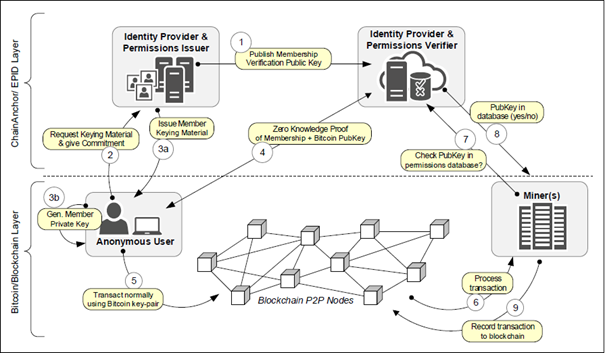
\includegraphics{anonymous_identities_for_permissioned_blockchains.png}

Privacy is established by spreading the non anonymous interaction of the user across multiple organizational entities, so that each entity only has access to a small part of the users non masked identity.
\begin{itemize}
\item \textbf{Permission Issuer:}
Knows each given users personal key pairs, but has no knowledge of their bitcoin keys.
\item \textbf{Permission Verifier:}
Knows each given user's membership key pairs and transactional key pairs, but has no knowledge of their personal key pairs used in obtaining group membership key pairs. However each user part of the same group will look the same to the verifier
\item \textbf{Additional Privacy:}
User is able to choose his own permission verification entity, so that the risk of collusion between parties is reduced immensely
\end{itemize}

\subsection{Assumptions about the underlying System}
\begin{itemize}
\item Permission issuer and permission verifier are separate entities and not in collusion (physically, operationally, legally separate entities)
\item User has Trusted Platform Module
\item Single permission issuer, however multiple permission verifier
\item During setup it is assumed that the permission issuer has a secure channel with mutual authentication to the permission verifier for transference of the membership verification public key
\item During user registration for permissioned groups it is assumed that the user and the permission issuer have a secure channel with mutual authentication
\end{itemize}
\subsection{Continuing Work}
In the coming months the authors are going to focus on supporting anonymous attribute groups in identity providers. These are called assertions in SAML2.0 or claims in OpenID-Connect and verification is obtained from external sources or attribute authorities. Furthermore they are working on implementing a RESTful design for their zero-knowledge proof protocol and support for Anti-Money Laundering (AML).


